\chapter{Experimente practice}

\section{Descrierea obiectelor}

Kitul de laborator pe care 'in ve'ti primi con'tine: rezistoare, surs'a de tensiune, multimetru, breadboard, fire de conexiune.

\subsection{Rezistoarele}

Ve'ti primi un set de 8 rezistoare (Fig. \ref{fig:4_rezistoare}). Rezistoarele primite au valoarea 'si toleran'ta codificate prin benzi colorate, conform Fig. \ref{fig:rezistente_cod_culori}.	

\begin{figure}[b]
	\centering
		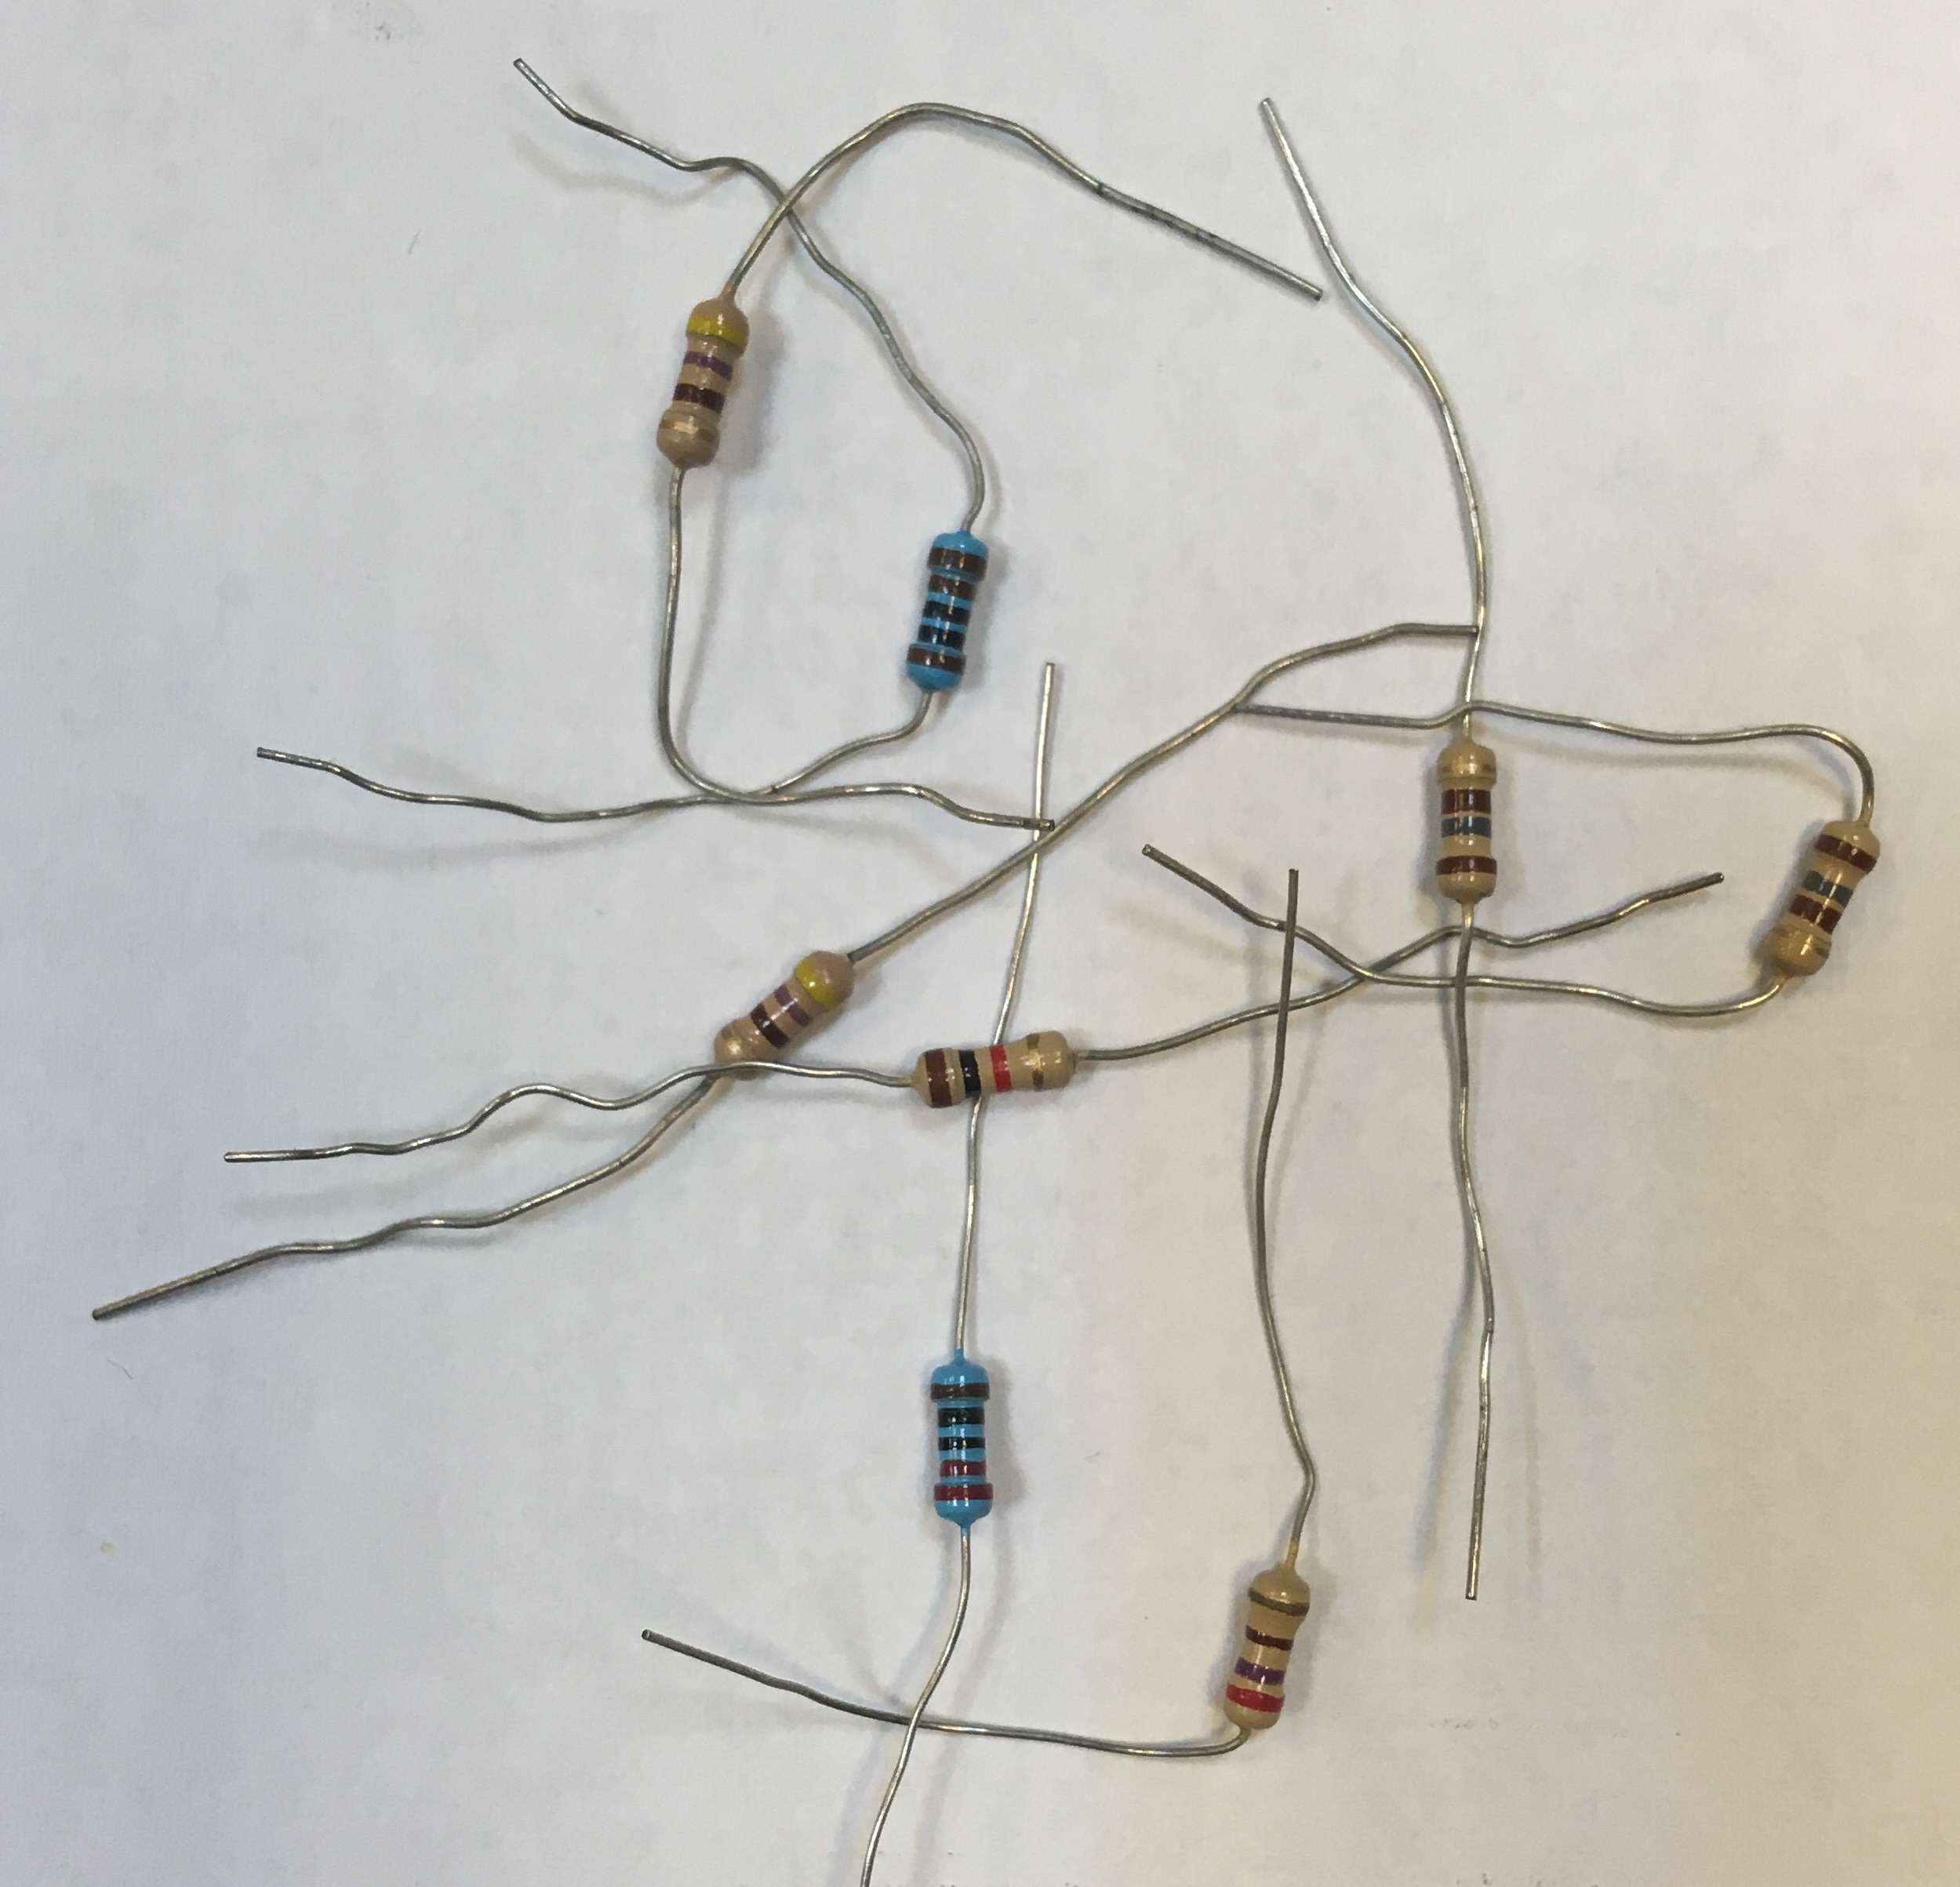
\includegraphics[width=0.35\textwidth]{figuri/4_rezistoare}
	\caption{Kit-ul de laborator -- rezistoare.}
	\label{fig:4_rezistoare}
\end{figure}
\begin{figure}
	\centering
		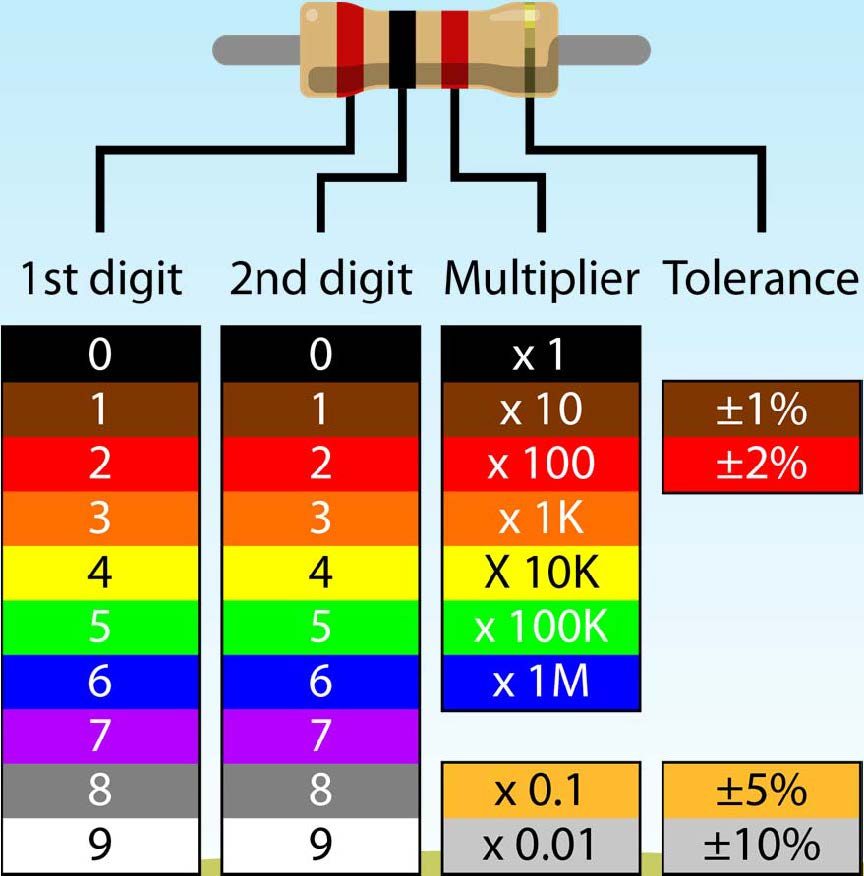
\includegraphics[width=0.6\textwidth]{figuri/rezistente_cod_culori}
	\caption{Codul de culori pentru un rezistor cu 4 benzi. Valoarea acestei rezisten'te este de 2 K$\Omega$, cu o toleran't'a de 5\%.}
	\label{fig:rezistente_cod_culori}
\end{figure}

\subsection{Sursa de tensiune}
\label{sectiune_sursa_tensiune}

Sursa de tensiune cu care se va lucra este cea din Fig. \ref{fig:4_sursa_tensiune}. Stabilirea tensiunii se face cu ajutorul a dou'a butoane rotative, unul pentru reglare grosier'a ('in dreapta, marcat cu \textit{COARSE}), cel'alalt pentru reglare mai fin'a ('in st\^anga, marcat cu \textit{FINE}). Tensiunea este afi'sat'a cu o singur'a zecimal'a, ceea ce ne determin'a s'a consider'am marginea erorii absolute a tensiunii de alimentare $U$ de $0.1$ V. 

Pentru mai multe informa'tii despre sursa de tensiune folosit'a 'in laborator consulta'ti manualul de utilizare \cite{PROTEK_Manuals}, disponibil 'si pe moodle.

\begin{figure}
	\centering
		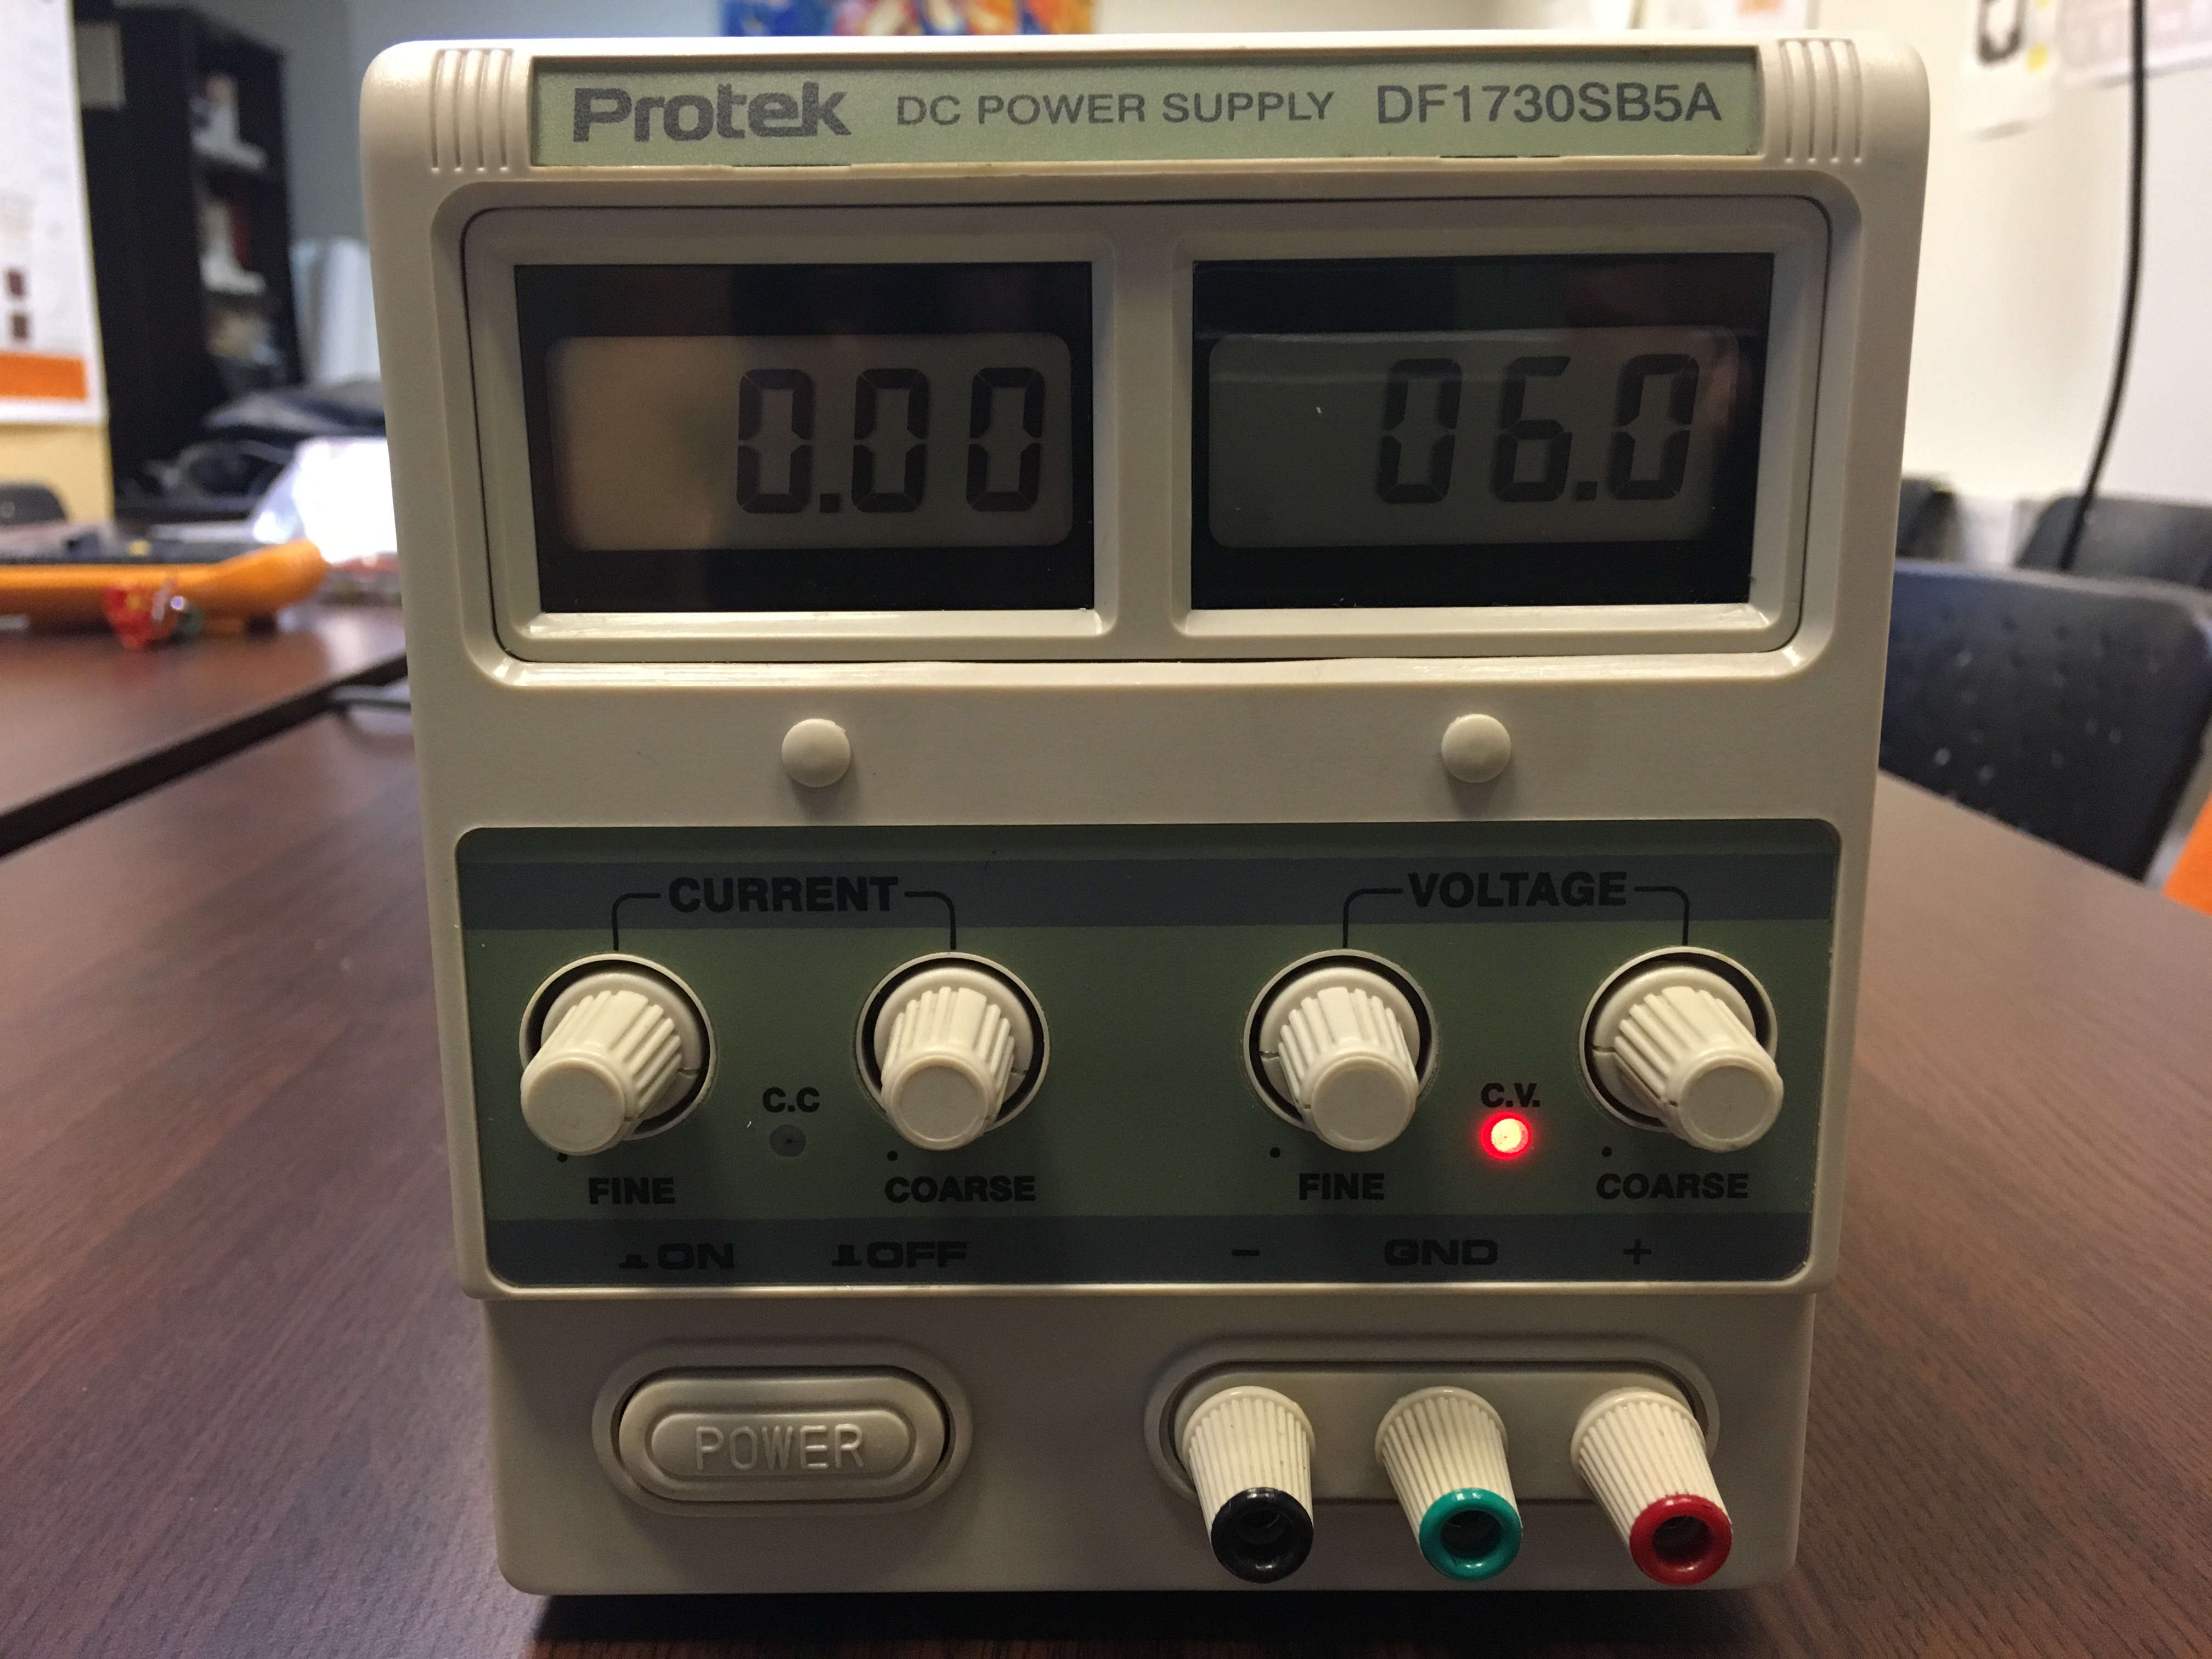
\includegraphics[width=0.5\textwidth]{figuri/4_sursa_tensiune}
	\caption{Kit-ul de laborator -- sursa de tensiune.}
	\label{fig:4_sursa_tensiune}
\end{figure}
\begin{figure}
	\centering
		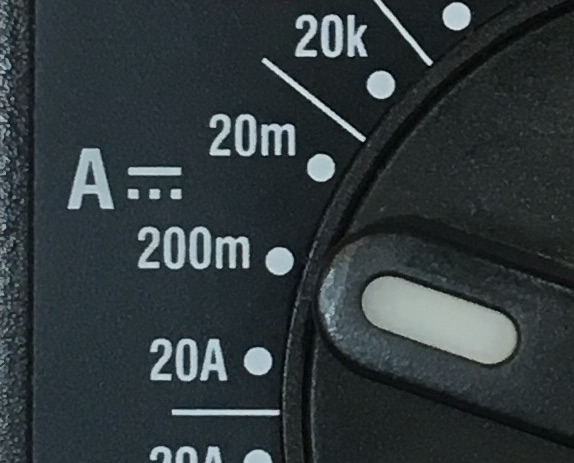
\includegraphics[width=0.2\textwidth]{figuri/4_multimetru_doar_curent}
		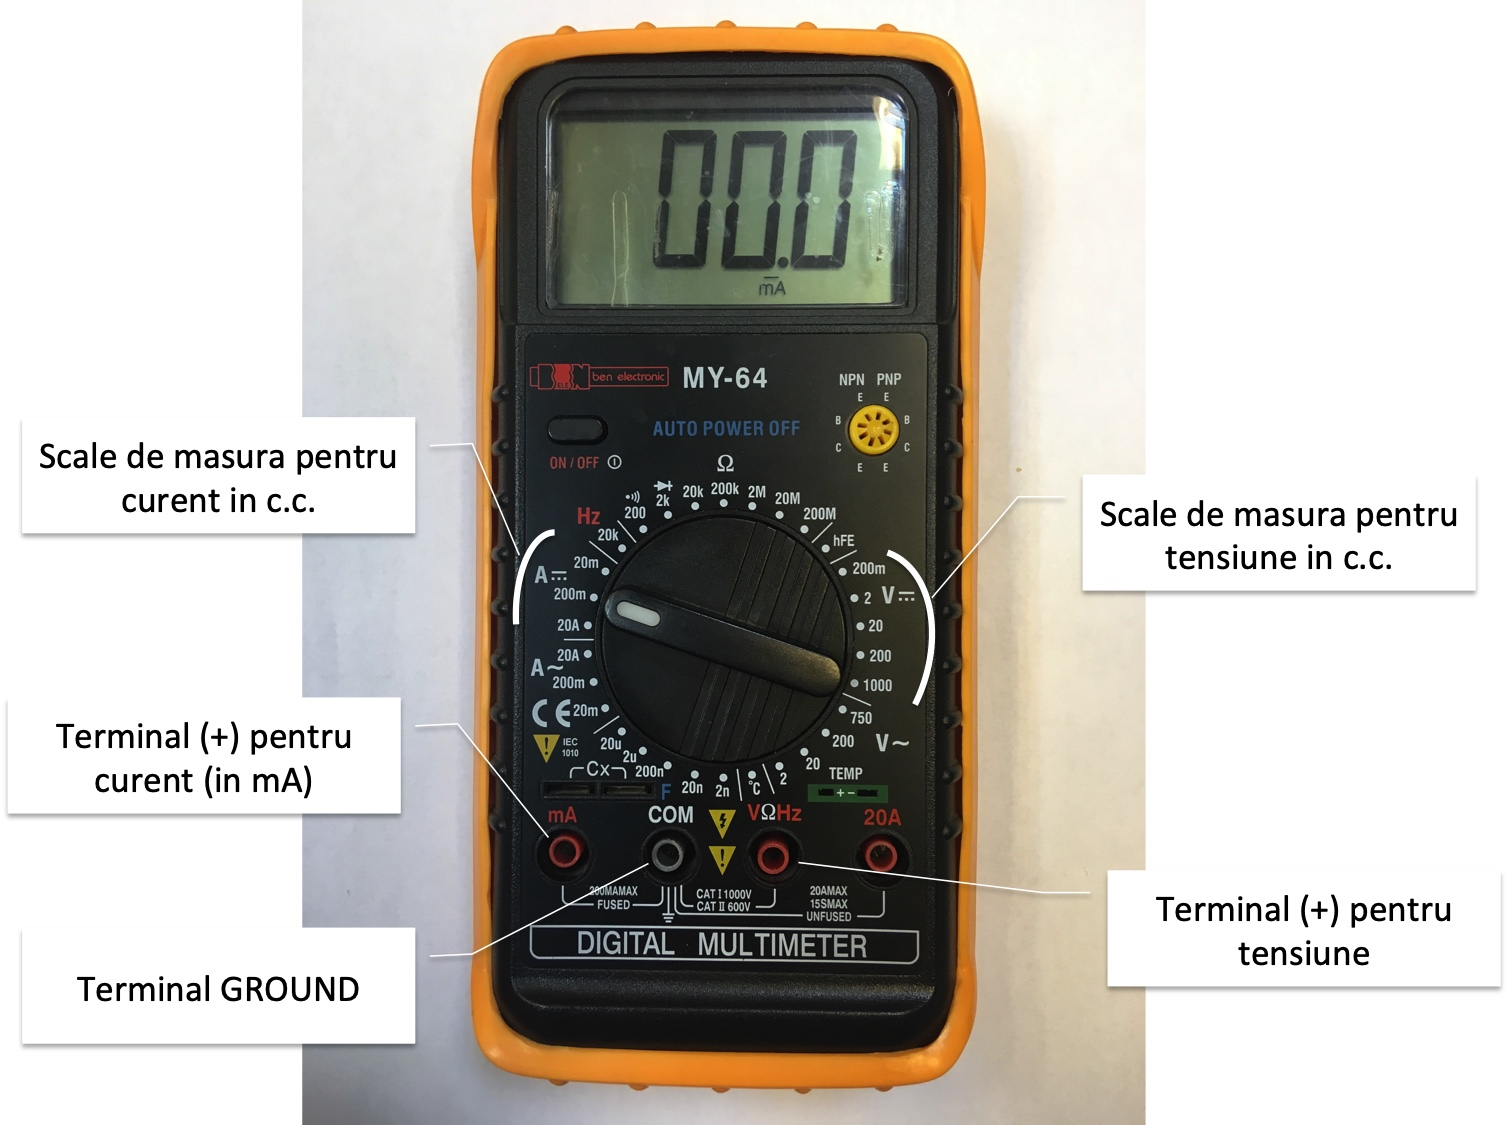
\includegraphics[width=0.5\textwidth]{figuri/4_multimetru_prel}
		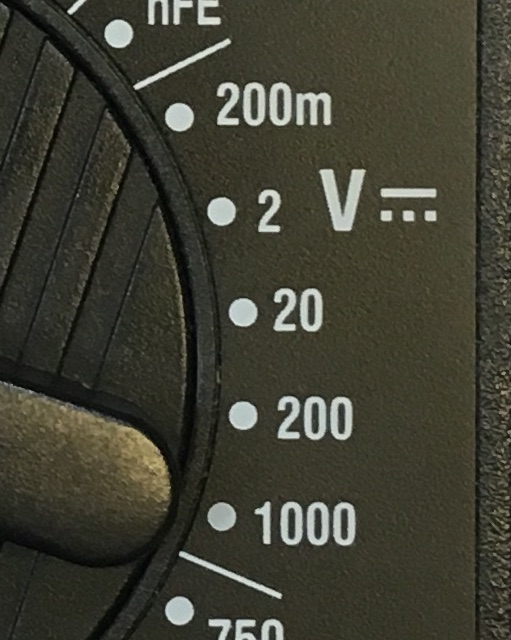
\includegraphics[width=0.2\textwidth]{figuri/4_multimetru_doar_tensiune}
	\caption{Kit-ul de laborator -- multimetru.}
	\label{fig:4_multimetru}
\end{figure}

\subsection{M'asurarea tensiunii 'si curentului}

Pentru m'asur'ari se va folosi un dispozitiv numit \textit{multimetru} (Fig. \ref{fig:4_multimetru}). Acest aparat poate m'asura diferite tipuri de m'arimi: curen'ti 'in c.c., rezisten'te, tensiuni 'in c.c., curen'ti 'in c.a., tensiuni 'in c.a., frecven'te. Pentru m'asurarea curen'tilor de c.c avem la dispozi'tie trei scale de m'arime: $20$ mA, $200$ mA, $20$ A. Pentru m'asurarea tensiunii 'in curent continuu exist'a cinci scale de m'arime: $200$ mV, $2$ V, $20$ V, $200$ V, $1000$ V. 

Precizia de m'asurare a fiec'arui aparat poate fi consultat'a 'in documenta'tie, de exemplu pentru multimetrul utilizat pentru m'asurarea tensiunii 'in curent continuu, informa'tia extras'a este 'in Fig. \ref{fig:acuratete_multimetru_tensiune}.
\begin{figure}
	\centering
		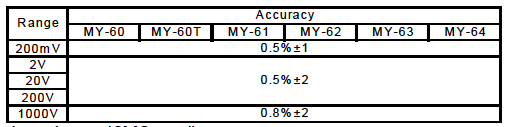
\includegraphics[width=0.7\textwidth]{figuri/acuratete_multimetru_tensiune}
	\caption{Precizia voltmetrului. Pentru scala de 2 V, precizia este de $0.5\%$ din valoarea m'asurat'a +2 zecimale, ceea ce 'inseamn'a o margine a erorii absolute de $\frac{0.5}{100}2+0.01=0.11 V$}.
	\label{fig:acuratete_multimetru_tensiune}
\end{figure}


M'asurarea unei m'arimi din circuit se face prin pozi'tionarea manetei rotative (Fig. \ref{fig:4_multimetru}) pe scala de m'arime (de ex. dac'a ne a'stept'am la un curent de aprox. 100 mA, atunci vom seta multimetrul 'in dreptul \textit{200m} ca 'in figura) 'si montarea corespunz'atoare a acestuia 'in circuit.

%Figura  \textcolor{red}{figura multimetru} sugereaz'a modul de reglare pentru a m'asura curentul de p\^n'a la 200 mA.

\begin{retine}
Ampermetrul se monteaz'a 'in serie cu latura pe care se dore'ste m'asurarea curentului. Voltmetrul se conecteaz'a 'intre cele dou'a noduri din circuit 'intre care se dore'ste m'asurarea tensiunii.

'In curent continuu este important modul de conectare a aparatului. M'arimile m'asurate reprezint'a valori fa't'a de un sens de referin't'a de la borna + (aici V) la borna -- (aici COM).
\end{retine}

Pute'ti g'asi mai multe informa'tii despre acest aparat de m'asur'a 'in documenta'tia disponibil'a online (\cite{multimeter_manual}) sau pe moodle.

\subsection{Realizarea interconexiunilor}

Asamblarea circuitului se face pe pl'acu'ta de baz'a, numit'a \textit{breabdoard}. Liniile galbene din Fig. \ref{fig:4_breadboard_prel} reprezint'a conexiuni, astfel 'inc\^at mai multe spa'tii reprezint'a acela'si nod.

\begin{figure}[!b]
	\centering
		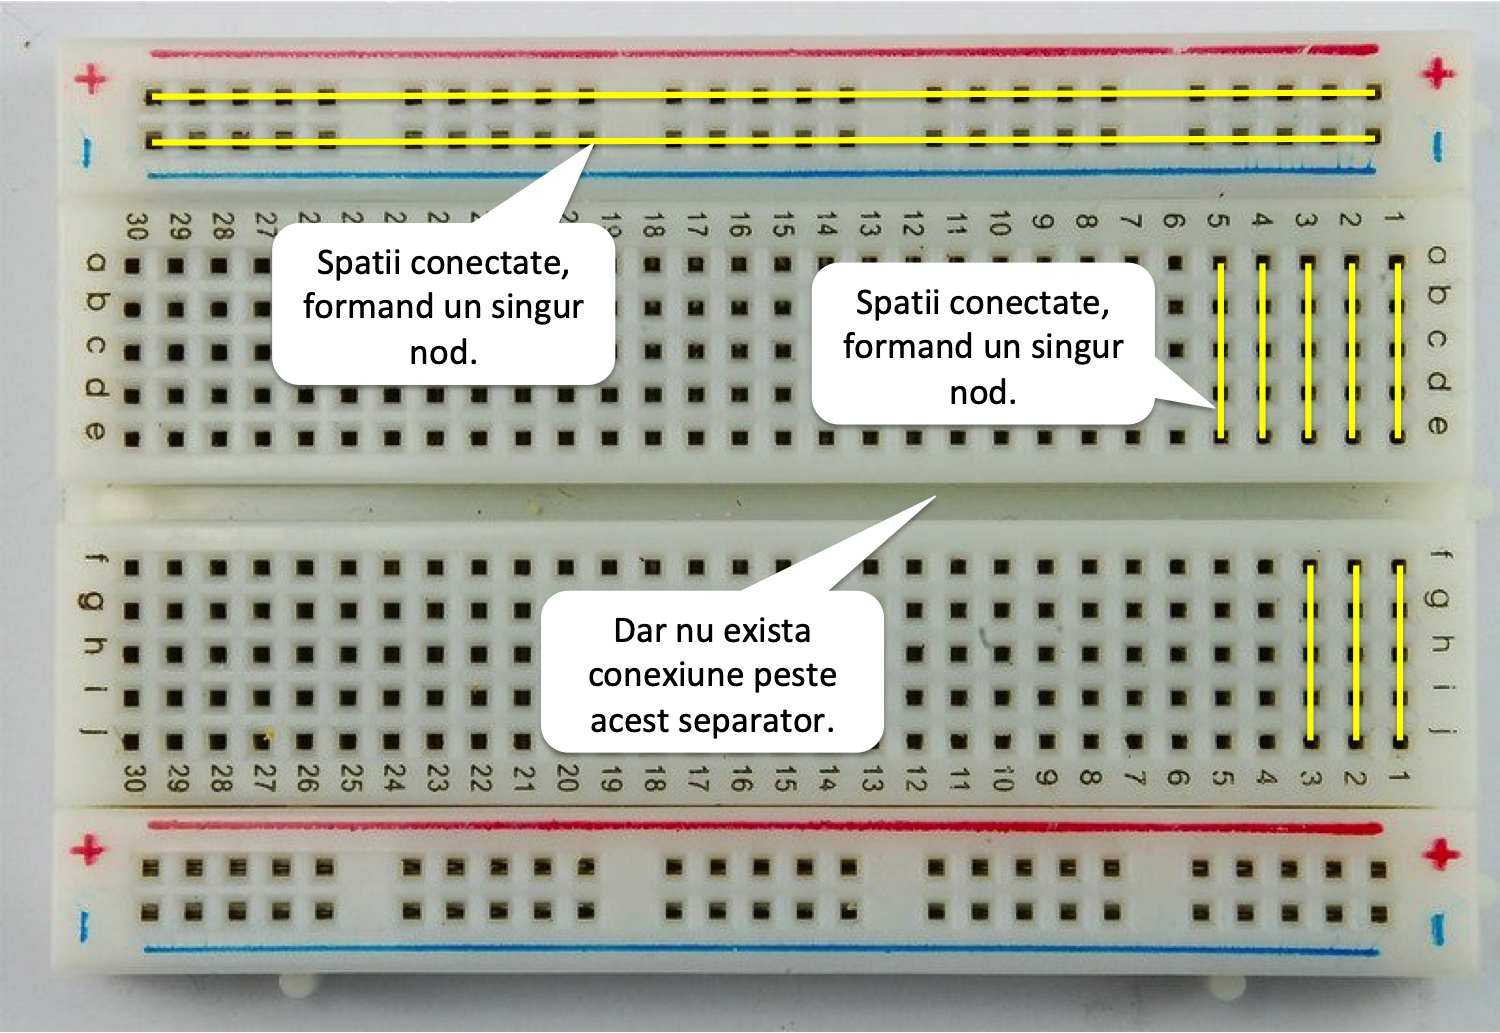
\includegraphics[width=0.5\textwidth]{figuri/4_breadboard_prel}
	\caption{Kit-ul de laborator -- placa \textit{breadboard}. Liniile galbene reprezint'a conexiuni, astfel 'inc\^at mai multe spa'tii formeaz'a acela'si nod.}
	\label{fig:4_breadboard_prel}
\end{figure}
\begin{figure}[!b]
	\centering
		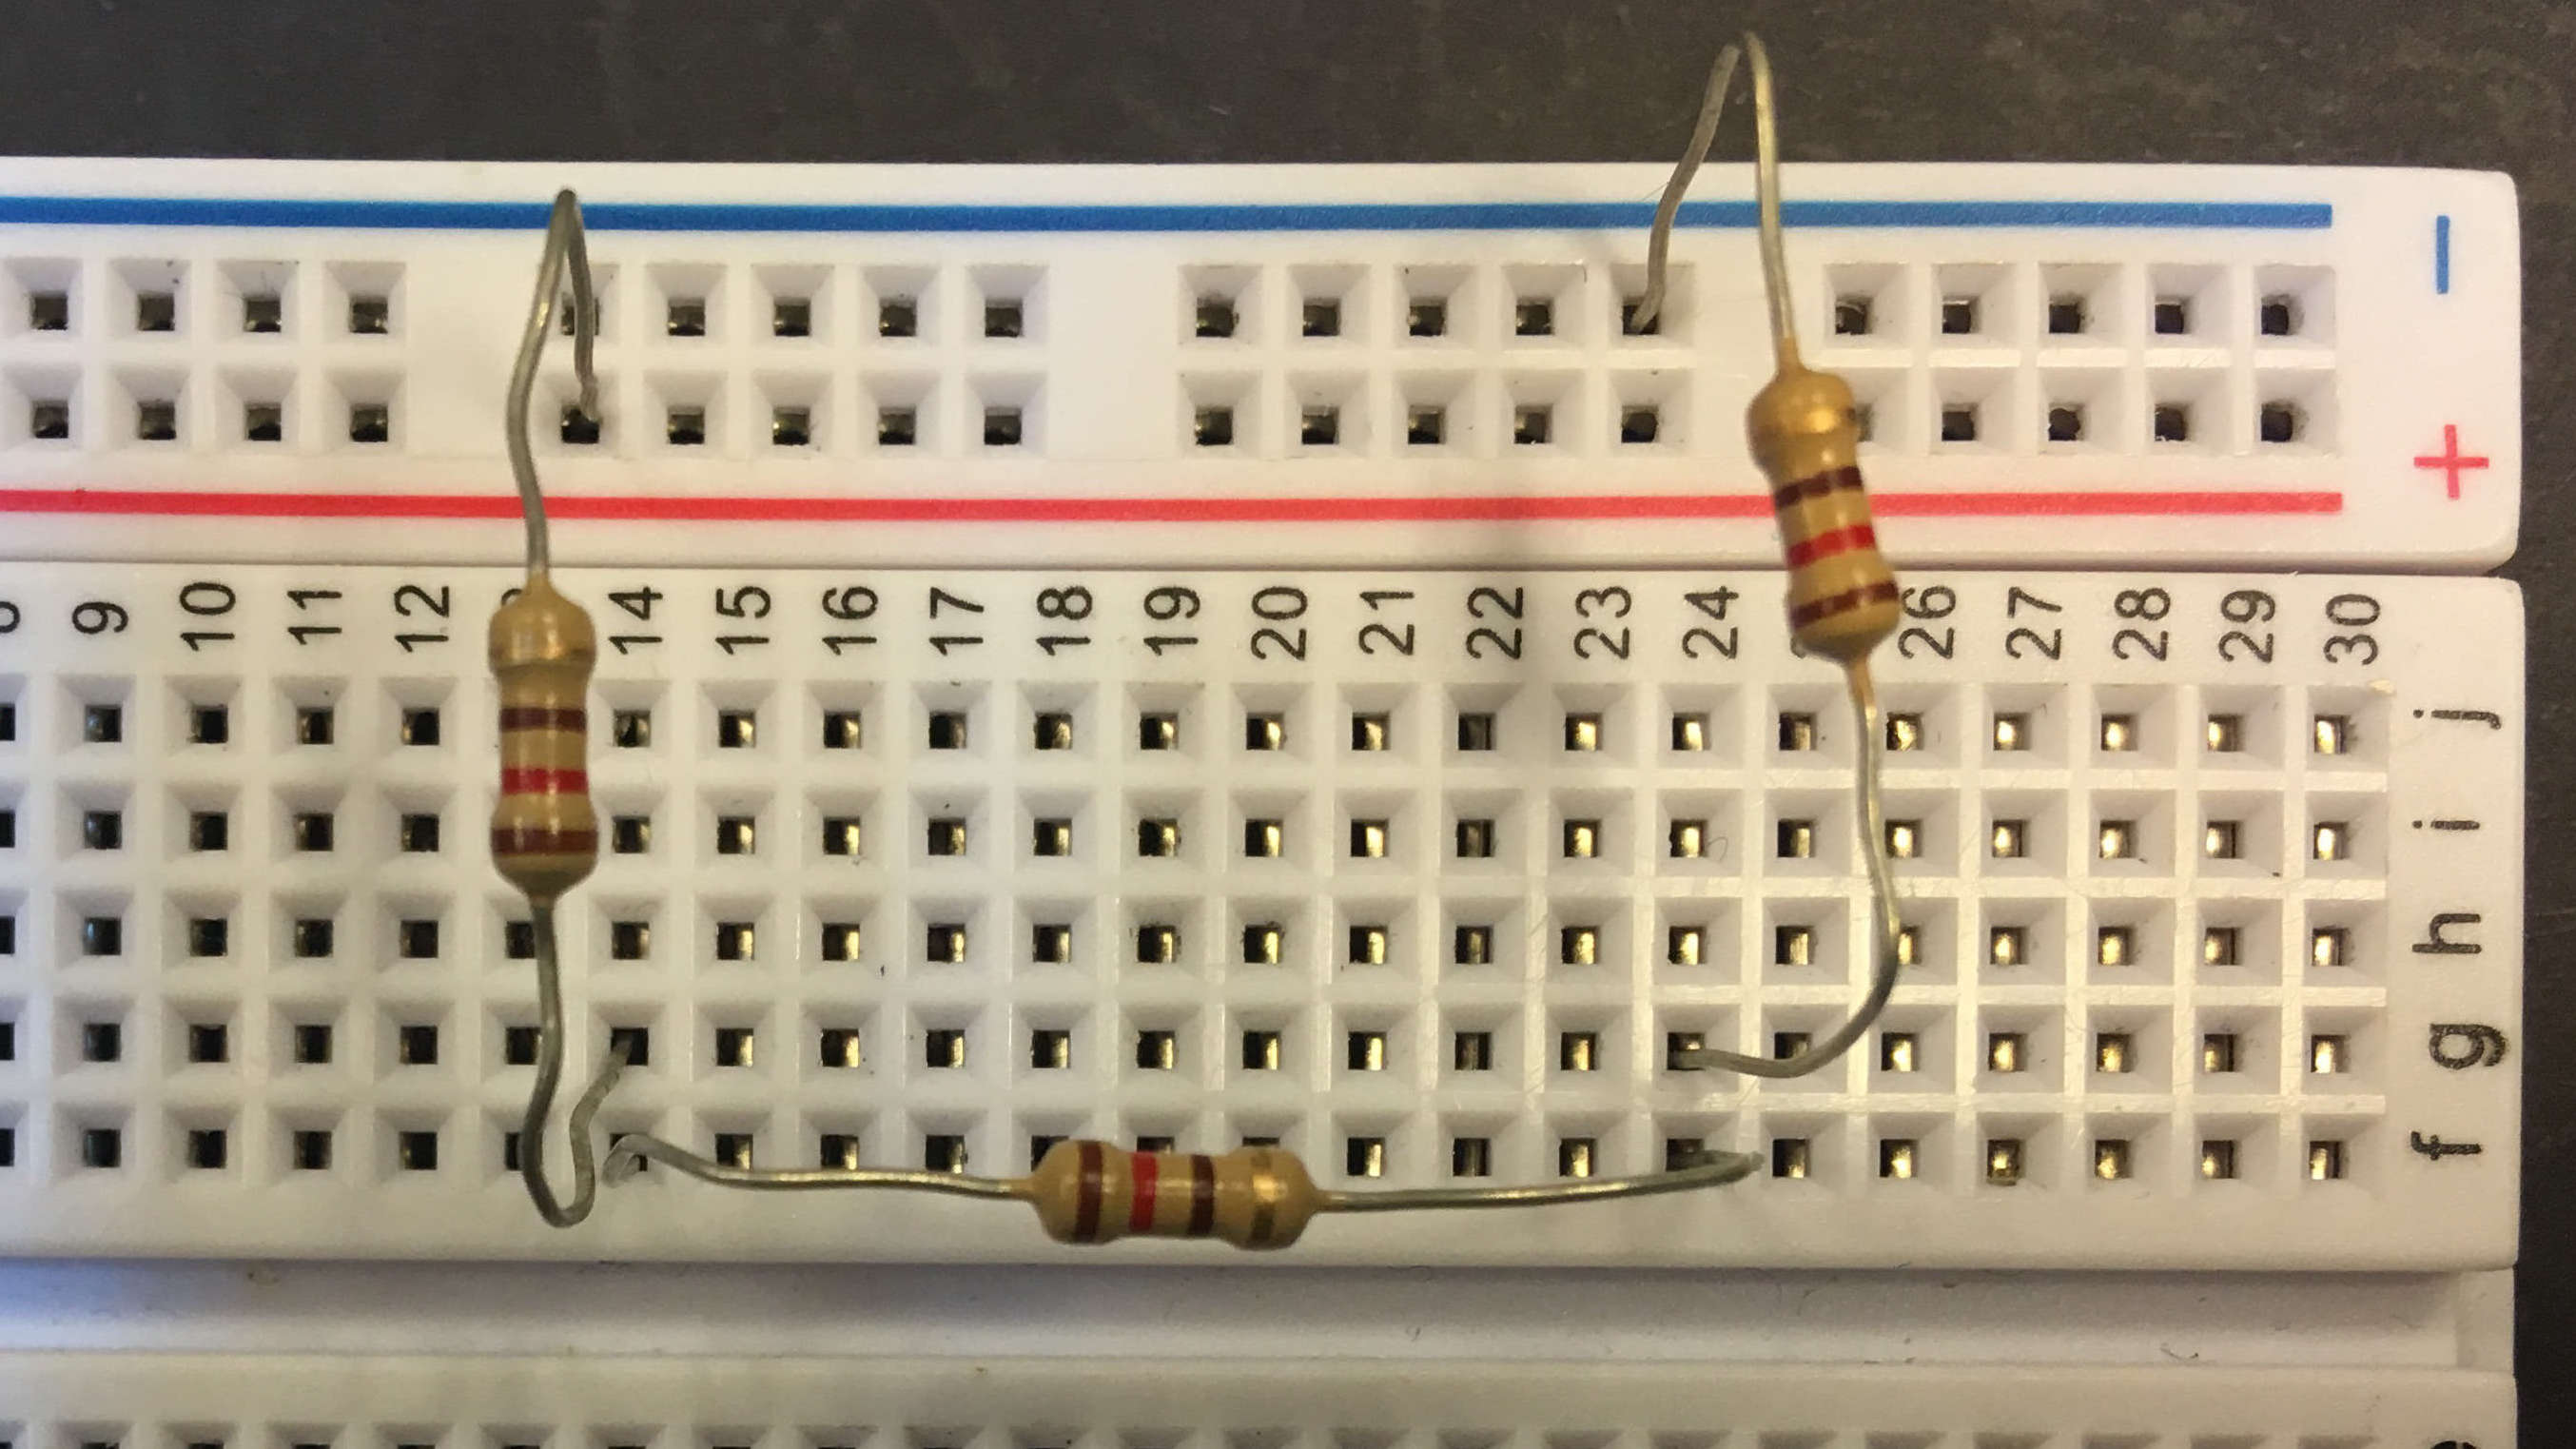
\includegraphics[width=0.6\textwidth]{figuri/4_divizor_gol_schema}
	\caption{Asamblarea circuitului divizor de tensiune 'in gol pe placa \textit{breadboard}.}
	\label{fig:4_divizor_gol_schema}
\end{figure}



\section{Lucrarea de laborator -- pas cu pas}

Experimentele pe care trebuie s'a le realiza'ti sunt descrise mai jos. 'In paralel cu ele trebuie s'a completa'ti chestionarul al treilea de pe moodle. Atentie, acest chestionar 'il pute'ti completa o singur'a dat'a, 'in timpul laboratorului.

\begin{exercise}[La laborator]
	Deschide'ti chestionarul de pe moodle.
\end{exercise}

\begin{figure}[!b]
	\centering
		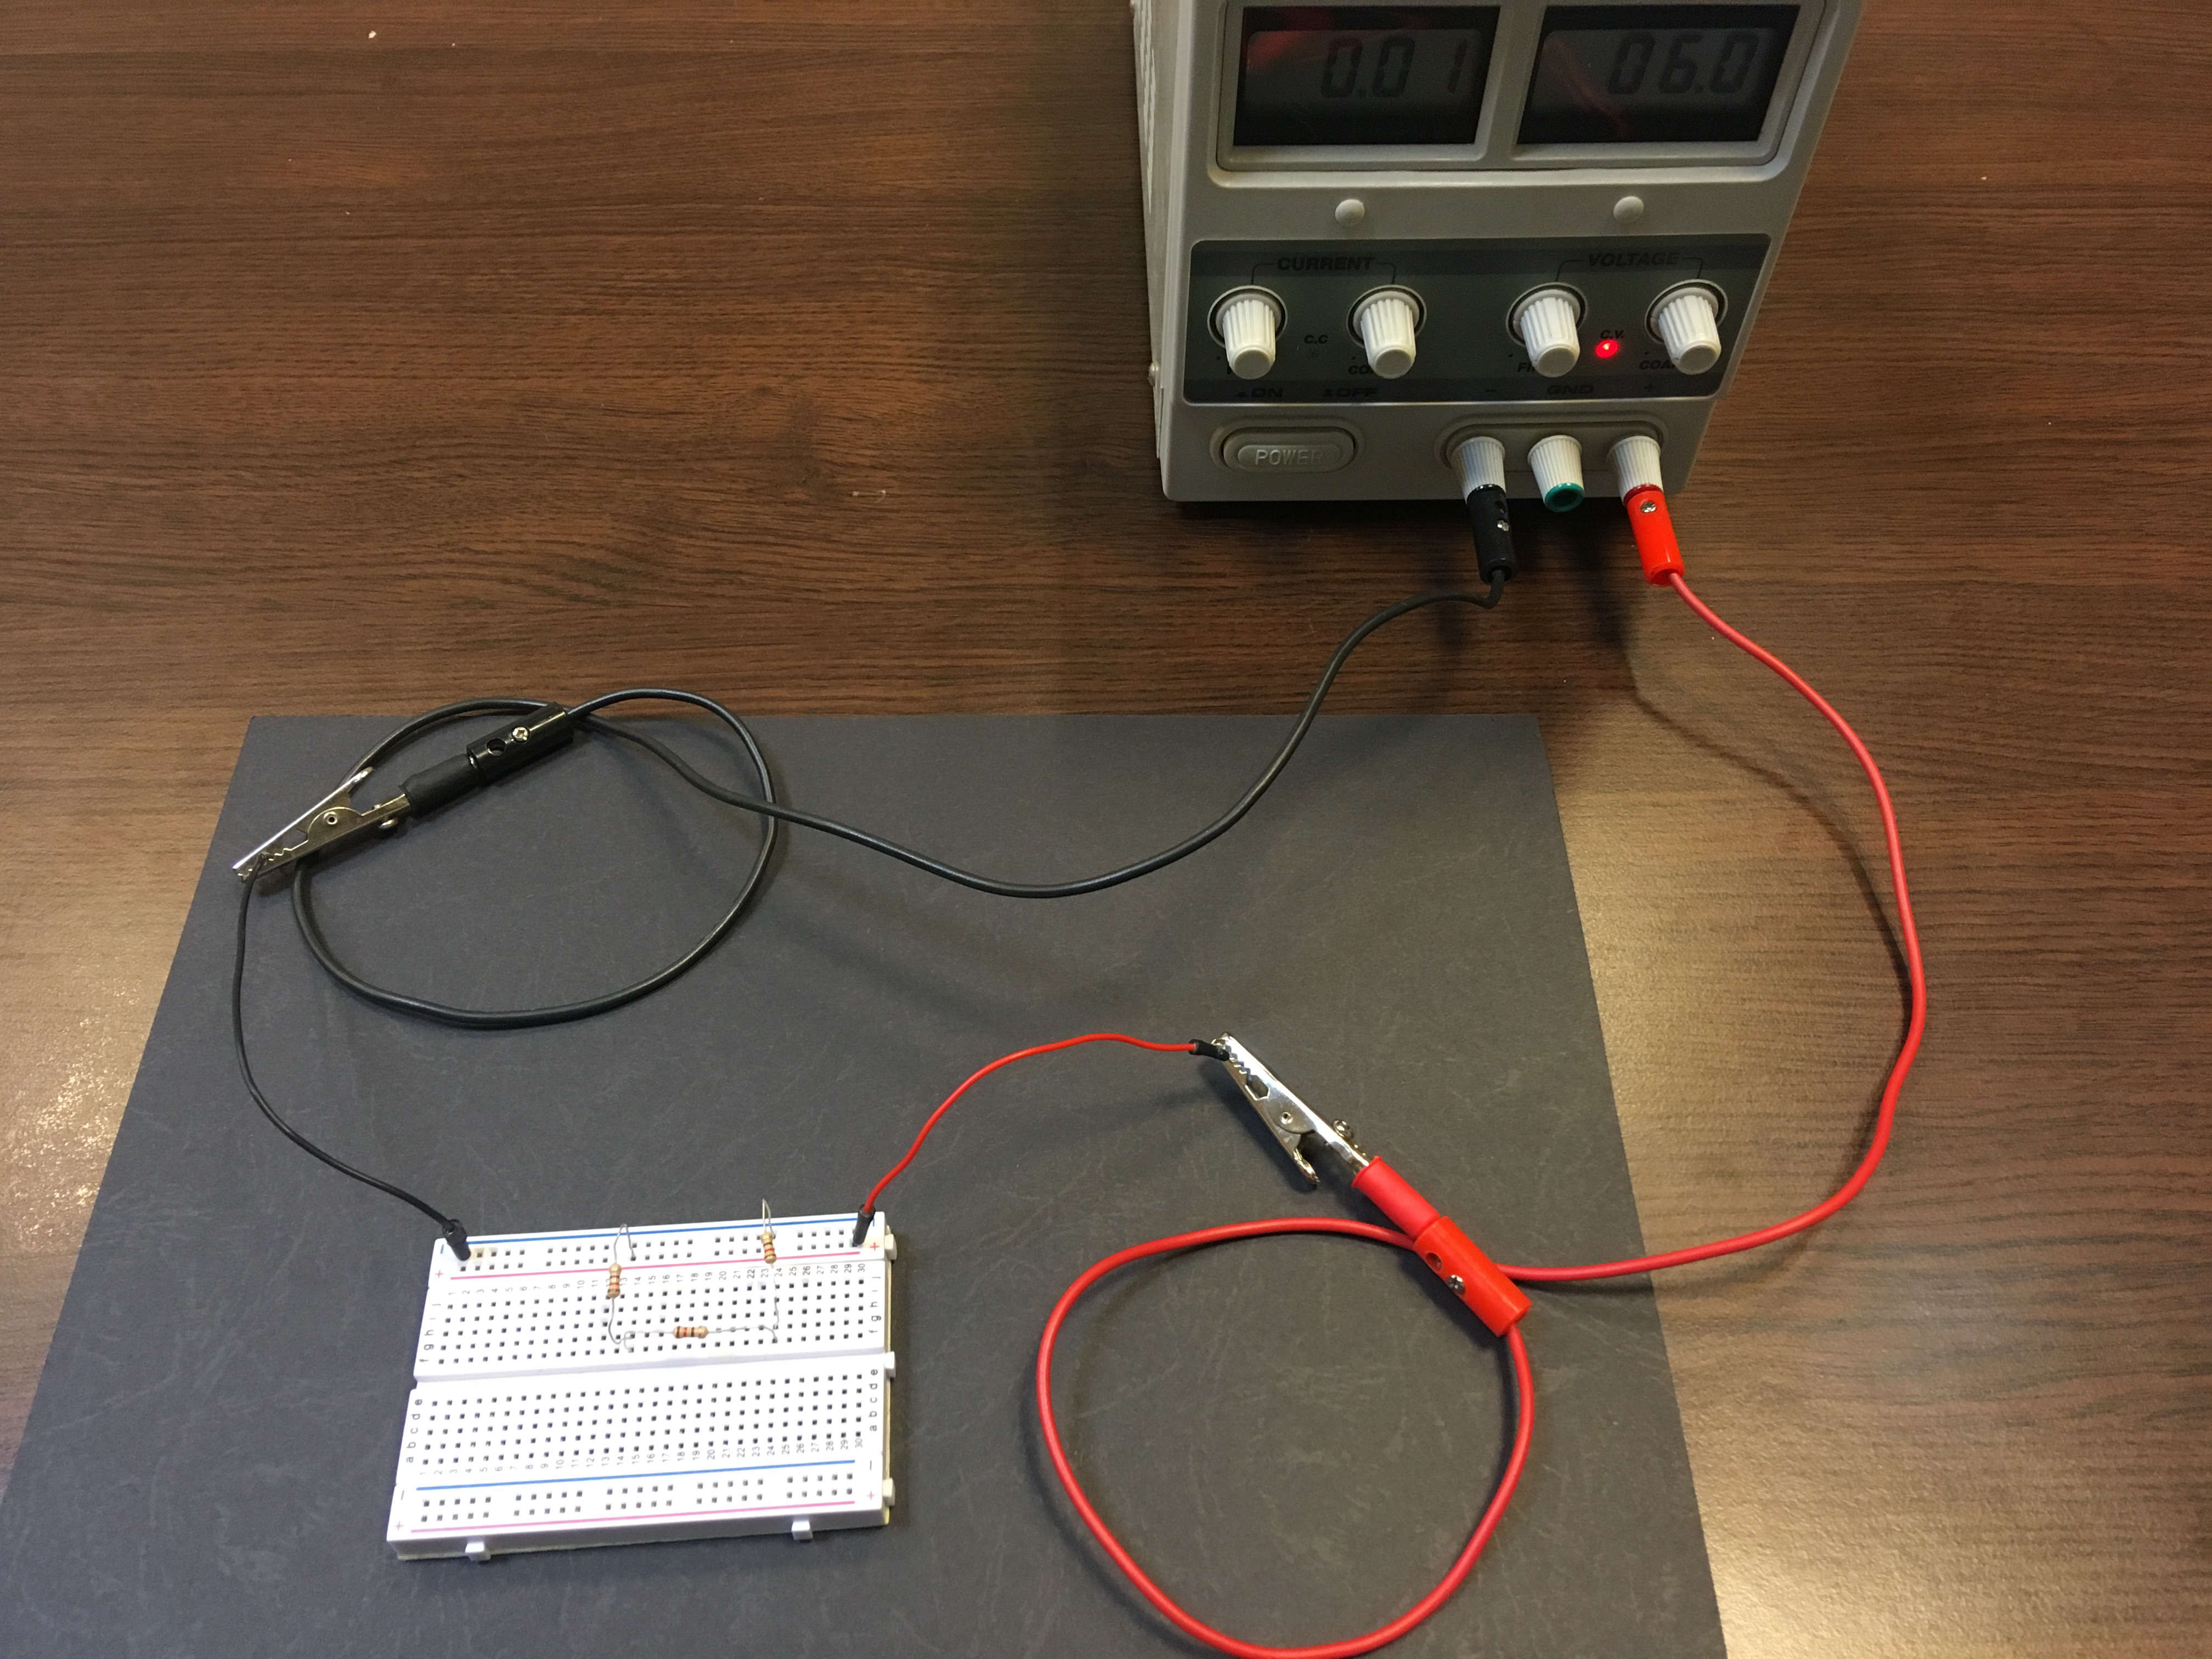
\includegraphics[width=0.5\textwidth]{figuri/4_divizor_gol_alimentat}
	\caption{Alimentarea divizorului de tensiune 'in gol cu o tensiune de 6 V.}
	\label{fig:4_divizor_gol_alimentat}
\end{figure}
\begin{figure}[!b]
	\centering
		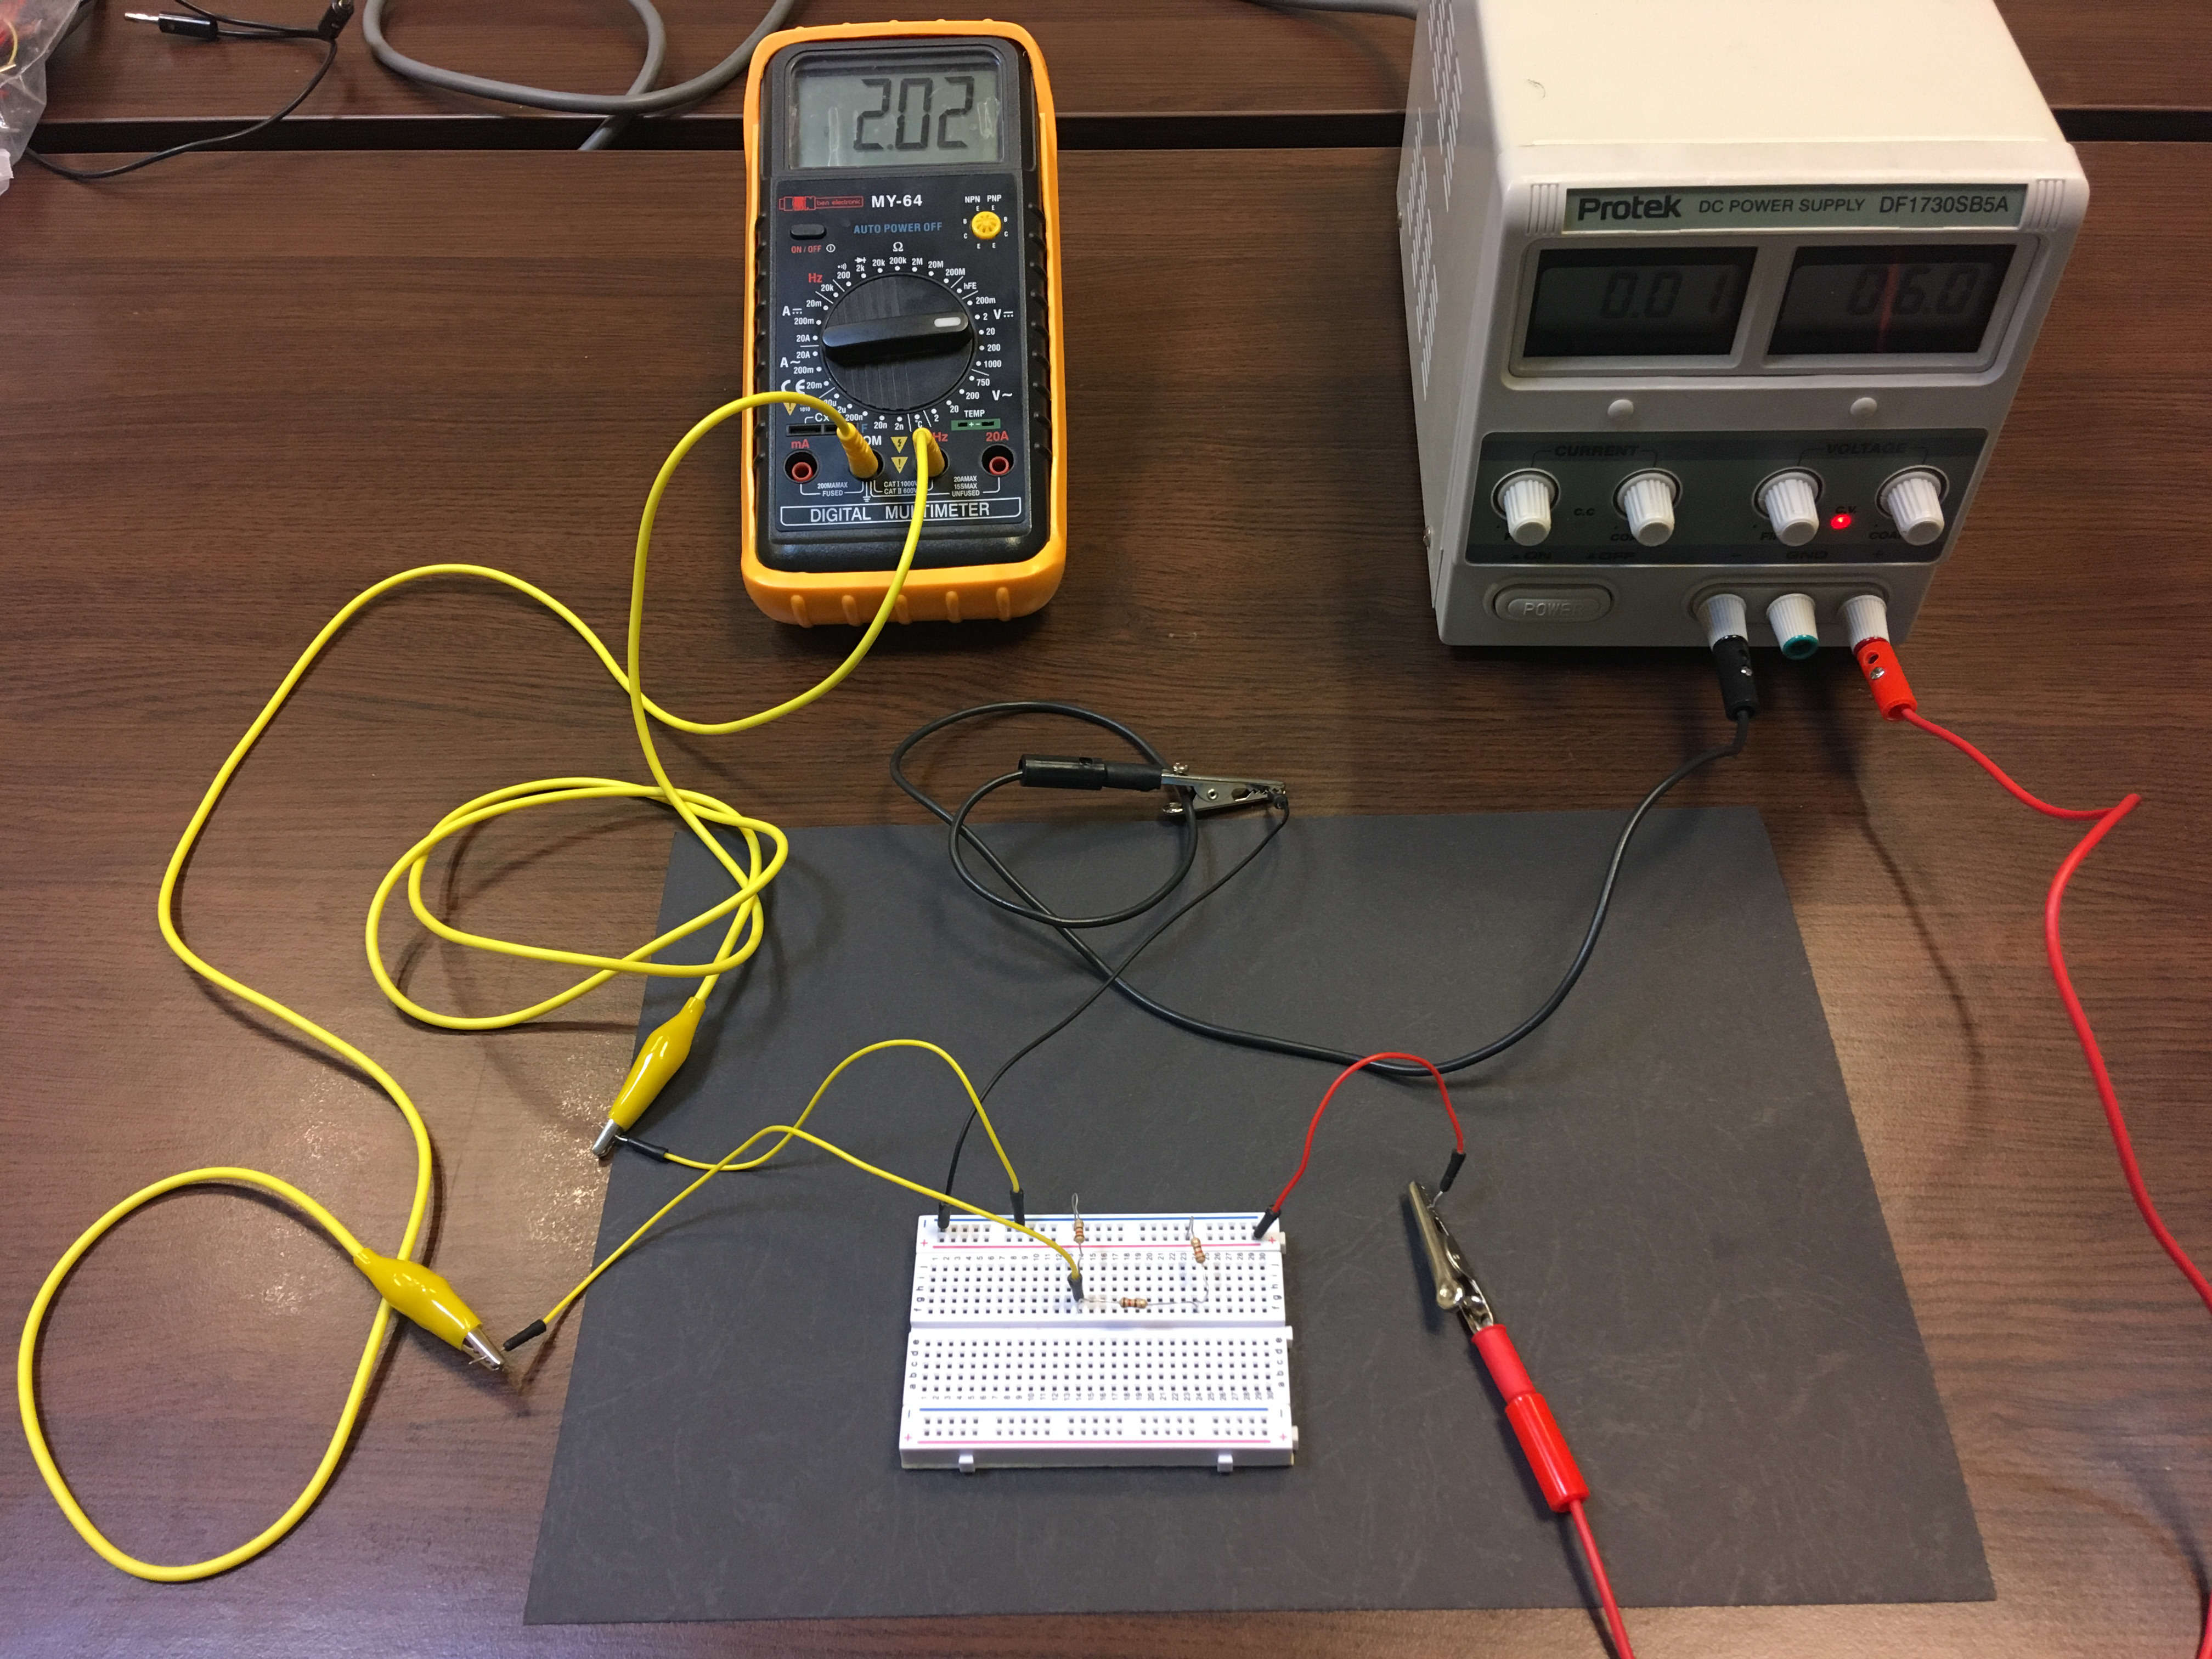
\includegraphics[width=0.5\textwidth]{figuri/4_divizor_gol_tensiune_iesire}
	\caption{M'asurarea tensiunii de ie'sire a divizorului de tensiune 'in gol.}
	\label{fig:4_divizor_gol_tensiune_iesire}
\end{figure}

Pentru realizarea lucr'arii practice de laborator, urma'ti pa'sii descri'si 'in continuare:

\subsection{Divizorul de tensiune 'in gol}

\begin{enumerate}
\item Determina'ti valorile rezisten'telor din setul primit 'si valorile toleran'telor lor, utiliz\^and codul culorilor din Fig. \ref{fig:rezistente_cod_culori}.
\item Alege'ti o combina'tie de valori ale rezisten'telor din setul primit, astfel 'inc\^at s'a crea'ti un divizor de tensiune cu 3. Desena'ti (pe foaie) schema de principiu a acestui divizor de tensiune, cu valori numerice 'si noduri etichetate. Indica'ti coresponden'ta cu rezistoarele $R_1$ 'si $R_2$ din schemele conceptuale din Sec'tiunea 2.
\item Asambla'ti circuitul divizorului de tensiune conform schemei concepute. Montajul rezistoarelor pe placa breadboard va fi similar cu cel din Fig. \ref{fig:4_divizor_gol_schema}.
\item Regla'ti sursa la valoarea stabilit'a, folosind cele dou'a butoane rotative, a'sa cum este descris 'in sec'tiunea \ref{sectiune_sursa_tensiune}.
\item Conecta'ti sursa de tensiune 'in circuit, dup'a verificarea corectitudinii montajului. Alimentarea circuitului de test reprezentat 'in Fig. \ref{fig:4_divizor_gol_schema} se face prin conectarea nodului din circuit $(n+)$ la terminalul $(+)$ al sursei (terminalul ro'su) 'si a nodului $(n-)$ la terminalul $(-)$ al sursei (terminalul negru) (Fig. \ref{fig:4_divizor_gol_alimentat}).
\item M'asura'ti tensiunea de ie'sire a divizorului, de la bornele rezistorului $R_2$. Folosi'ti maneta rotativ'a a multimetrului pentru a seta scala de m'arime la 20 V 'si conecta'ti aparatul 'in paralel cu $R_2$ ('in exemplul nostru 'intre nodurile (24) 'si (n-)): nodul (24) se conecteaz'a la terminalul notat cu $V$ al aparatului, iar nodul $(n-)$ se conecteaz'a la terminalul notat \textit{COM} (\textit{ground}) (Fig. \ref{fig:4_divizor_gol_tensiune_iesire}).

\subsection{Divizorul de tensiune 'in sarcin'a}

\item Conecta'ti la ie'sirea divizorului de tensiune o rezisten't'a de sarcin'a din setul primit. M'asura'ti tensiunea de ie'sire din divizor 'in acest caz.

\subsection{Puntea rezistiv'a}

\item Conecta'ti 'n paralel cu divizorul ini'tial (format din $R_1$, $R_2$) un divizor $R_3$, $R_4$ astfel 'inc\^at s'a se formeze o punte echilibrat'a. 
\item M'asura'ti tensiunea 'intre nodurile $(a)$ 'si $(b)$ ale pun'tii.
\item M'asura'ti c\^at este curentul absorbit de punte.

\subsection{Finalizarea laboratorului}

\item Revede'ti r'aspunsurile completate 'in chestionarul de laborator, finaliza'ti 'si 'inchide'ti chestionarul.
\end{enumerate}





